\documentclass[10pt]{beamer}

% \usepackage{define}
\usepackage{animate}

\usetheme{CCFD}
\usepackage{color}
\definecolor{gray97}{gray}{.90}
\definecolor{gray75}{gray}{.75}
\usepackage{listings}
\lstset{frame=Ltb,
     framerule=0pt,
     aboveskip=0cm,
     framextopmargin=0pt,
     framexbottommargin=0pt,
     framexleftmargin=0cm,
     framesep=0pt,
     rulesep=0pt,
     backgroundcolor=\color{gray97},
     rulesepcolor=\color{black},
     language=C,
           basicstyle=\ttfamily\scriptsize,
           keywordstyle=\color{blue}\ttfamily,
           stringstyle=\color{red}\ttfamily,
           commentstyle=\color{green}\ttfamily,
          breaklines=true,
          }
\lstdefinestyle{consol}
   {basicstyle=\scriptsize\bf\ttfamily,
    backgroundcolor=\color{gray75},
}
\resetcounteronoverlays{lstnumber}

\newcommand{\tabitem}{%
  \usebeamertemplate{itemize item}\hspace*{\labelsep}}

\usepackage{tikz}
\usetikzlibrary{calc,shapes,arrows.meta}

\eventtitle{Computer Science I}
\title{Lecture 6\\Pointers and addresses}
\date{}

\setbeamertemplate{blocks}[rounded][shadow=true]
\setbeamertemplate{navigation symbols}[]

\newcommand\aeDiagonalNumber{100}
\newcommand\memorySixtyFive{%%' 
  \begin{minipage}{2.75cm}
    \centering
    char `a' in memory\par       
    (65 = ascii code)
  \end{minipage}}

\begin{document}

\frame{
%\framesubtitle{What is your pointer, what is your address?}
    \titlepage
}

\begin{frame}
  \frametitle{Test is coming}
  \begin{itemize}
    \item Data types
    \item Functions
    \item I/O operations
    \item Branching (if, switch)
    \item Loops
  \end{itemize}
  
  Have a look at the example tests!
\end{frame}


\section{Memory}

\begin{frame}[fragile]
  \frametitle{The memory}
  \framesubtitle{Is where variables live}
  \vspace{-0.3cm}
  \begin{columns}
    \begin{column}{0.7\textwidth}
      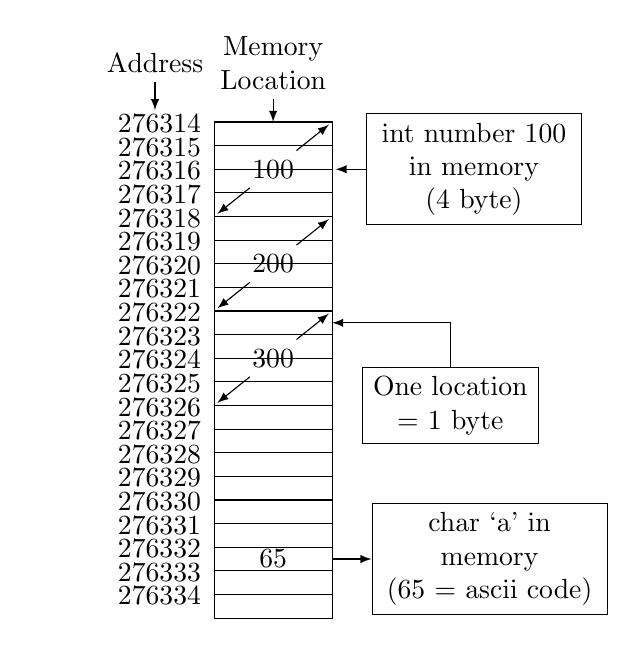
\begin{tikzpicture}[x=1.5cm,y=0.3cm]
  %% Building the boxes representing memory locations
  \foreach \x in {0,1,...,20}
  {
    \node[inner sep=1pt] (BL\x) at (0,-\x)   {};
    \node[inner sep=1pt] (UR\x) at (1,-\x+1) {};
    \node (MM\x) at ($(BL\x)!0.5!(UR\x)$) {};
    \draw (BL\x) rectangle (UR\x);
    \edef\memoryNumber{\number\numexpr276314+\x\relax}
    \node[anchor=south east] at (BL\x.north west) {\memoryNumber};
  }

  %% Label columns:
  \node (MEMLOC) at ($(MM0)+(0.0,0.9cm)$) { \parbox{2cm}{\centering Memory Location} };
  \node (ADDRESS) at ($(MEMLOC)-(1.0,0)$) {\parbox{3cm}{\centering Address} };
  \draw [-latex] (MEMLOC) -- ($(MM0|-UR0)+(0.0,0)$);
  \draw [-latex] (ADDRESS) -- ($(MM0|-UR0)-(1,-0.5)$);

  %% Drawing arrows spanning memory locations
  \foreach \x/\y in {3/0, 7/4, 11/8}
  {
    \node (M\x-\y) at ($(BL\x)!0.5!(UR\y)$) {\aeDiagonalNumber};
    \xdef\aeDiagonalNumber{\number\numexpr\aeDiagonalNumber+100\relax}
    \draw[-latex]  (M\x-\y) -- (BL\x) ; 
    \draw[-latex]  (M\x-\y) -- (UR\y) ;
  }

  %% Adding content to memory location "18"
  \node at (MM18) {65};
  \node (RHS18) at (MM18-|UR18) {};
  %% Adding a side note to memory location "18"
  \node[draw,anchor=west] (BOX18) at ($(RHS18)+(0.5cm,0)$) {\memorySixtyFive};
  \draw [-latex] (RHS18.center) -- (BOX18);

  %%
  \node [draw](1byte) at ($(UR12)+(1,0)$) { \parbox{2cm}{\centering One location = 1 byte}};
  \path [draw,-latex] (1byte) -- ($(1byte|-UR8)-(0,0.5)$) -- ($(UR8)-(0,0.5)$);

  \node [draw](4byte) at ($(UR2)+(1.2,0)$) { \parbox{2.5cm}{\centering int number 100\\ in memory \\ (4 byte)}};
  \path [draw,-latex] (4byte) -- (UR2);

\end{tikzpicture}
    \end{column}
    \begin{column}{0.4\textwidth}
\begin{lstlisting}
...
int a=100;
int b=200;
int c=300;
char d='a';
...
\end{lstlisting}
\begin{itemize}
  \item Memory is continous
  \item All variables are stored in memory
  \item ... and functions
\end{itemize}
    \end{column}
  \end{columns}
\end{frame}

\section{Pointers}

\begin{frame}[fragile]
  \frametitle{New data types - pointers}
  \framesubtitle{declared with a *}
  \begin{itemize}
    \item For every type there is a pointer to it
    \item Use *
    \item Pointers are used to store \textbf{addresses} of variables
    \item Reside in memory, as any other variable
  \end{itemize}
  
\begin{lstlisting}
int *pi;
float *pf;
double *pd;
char *pc;
void *pv;
\end{lstlisting}
But also Pointer to pointer ...
\begin{lstlisting}
int **ppi;
float ***pf;
...
void **pv;
\end{lstlisting}
\end{frame}

\begin{frame}[fragile]
  \frametitle{Pointers}
  \framesubtitle{sizeof}
  \begin{columns}
    \begin{column}{0.4\textwidth}
    \begin{itemize}
    \item What is \textit{sizeof(int*)}
    \item and \textit{sizeof(double*)}
    \item Examples follow
    \item Depands on a system ...
    \end{itemize}
\begin{lstlisting}
int a=400;
int *p = 10; //p points to memory address 10, can we access it?
\end{lstlisting}
    \end{column}
    \begin{column}{0.7\textwidth}
      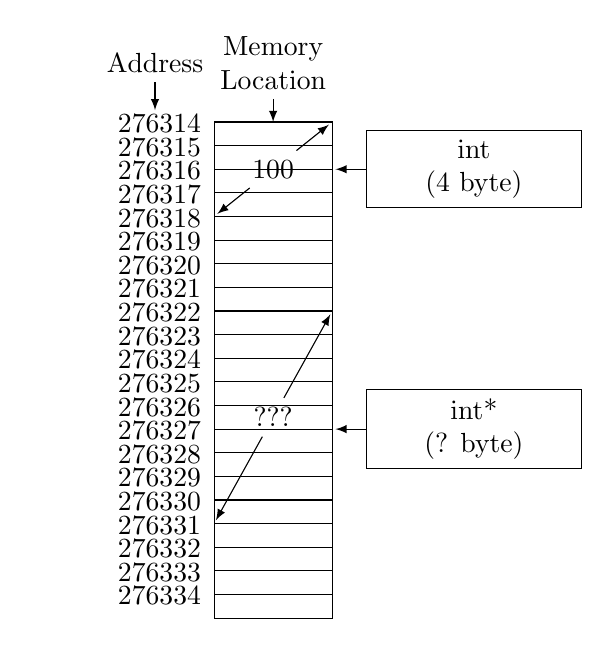
\begin{tikzpicture}[x=1.5cm,y=0.3cm]
  %% Building the boxes representing memory locations
  \foreach \x in {0,1,...,20}
  {
    \node[inner sep=1pt] (BL\x) at (0,-\x)   {};
    \node[inner sep=1pt] (UR\x) at (1,-\x+1) {};
    \node (MM\x) at ($(BL\x)!0.5!(UR\x)$) {};
    \draw (BL\x) rectangle (UR\x);
    \edef\memoryNumber{\number\numexpr276314+\x\relax}
    \node[anchor=south east] at (BL\x.north west) {\memoryNumber};
  }

  %% Label columns:
  \node (MEMLOC) at ($(MM0)+(0.0,0.9cm)$) { \parbox{2cm}{\centering Memory Location} };
  \node (ADDRESS) at ($(MEMLOC)-(1.0,0)$) {\parbox{3cm}{\centering Address} };
  \draw [-latex] (MEMLOC) -- ($(MM0|-UR0)+(0.0,0)$);
  \draw [-latex] (ADDRESS) -- ($(MM0|-UR0)-(1,-0.5)$);

  %% Drawing arrows spanning memory locations
  \foreach \x/\y in {3/0}
  {
    \node (M\x-\y) at ($(BL\x)!0.5!(UR\y)$) {\aeDiagonalNumber};
    \xdef\aeDiagonalNumber{\number\numexpr\aeDiagonalNumber+100\relax}
    \draw[-latex]  (M\x-\y) -- (BL\x) ; 
    \draw[-latex]  (M\x-\y) -- (UR\y) ;
  }

  \foreach \x/\y in {16/8}
  {
    \node (M\x-\y) at ($(BL\x)!0.5!(UR\y)$) {???};
    \draw[-latex]  (M\x-\y) -- (BL\x) ; 
    \draw[-latex]  (M\x-\y) -- (UR\y) ;
  }

  \node [draw](4byte) at ($(UR2)+(1.2,0)$) { \parbox{2.5cm}{\centering int \\ (4 byte)}};
  \path [draw,-latex] (4byte) -- (UR2);
  
  \node [draw](4byte) at ($(UR13)+(1.2,0)$) { \parbox{2.5cm}{\centering int* \\ (? byte)}};
  \path [draw,-latex] (4byte) -- (UR13);

\end{tikzpicture}
    \end{column}
  \end{columns}

\end{frame}

\begin{frame}[fragile]
  \frametitle{Retrieve the address}
  \framesubtitle{The \& operator}
    \begin{columns}
    \begin{column}{0.55\textwidth}
    \begin{itemize}
    \item Remember the \textit{scanf()}?
    \item \& is used to retrieve an address of a variable in memory
    \item \& returns the beginning of the space in memory where a variable is
    \end{itemize}
\begin{lstlisting}
int satan=2;//this is an evil int
int *p = &a; //p stores adress of s
\end{lstlisting}
    \end{column}
    \begin{column}{0.7\textwidth}
      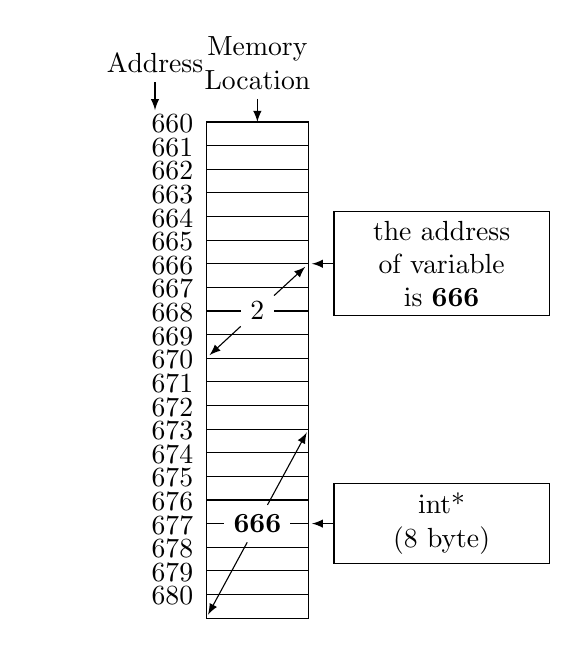
\begin{tikzpicture}[x=1.3cm,y=0.3cm]
  %% Building the boxes representing memory locations
  \foreach \x in {0,1,...,20}
  {
    \node[inner sep=1pt] (BL\x) at (0,-\x)   {};
    \node[inner sep=1pt] (UR\x) at (1,-\x+1) {};
    \node (MM\x) at ($(BL\x)!0.5!(UR\x)$) {};
    \draw (BL\x) rectangle (UR\x);
    \edef\memoryNumber{\number\numexpr660+\x\relax}
    \node[anchor=south east] at (BL\x.north west) {\memoryNumber};
  }

  %% Label columns:
  \node (MEMLOC) at ($(MM0)+(0.0,0.9cm)$) { \parbox{2cm}{\centering Memory Location} };
  \node (ADDRESS) at ($(MEMLOC)-(1.0,0)$) {\parbox{3cm}{\centering Address} };
  \draw [-latex] (MEMLOC) -- ($(MM0|-UR0)+(0.0,0)$);
  \draw [-latex] (ADDRESS) -- ($(MM0|-UR0)-(1,-0.5)$);

  %% Drawing arrows spanning memory locations
  \foreach \x/\y in {9/6}
  {
    \node[fill=white] (M\x-\y) at ($(BL\x)!0.5!(UR\y)$) {2};
    \draw[-latex]  (M\x-\y) -- (BL\x) ; 
    \draw[-latex]  (M\x-\y) -- (UR\y) ;
  }

  \foreach \x/\y in {20/13}
  {
    \node [fill=white] (M\x-\y) at ($(BL\x)!0.5!(UR\y)$) {\textbf{666}};
    \draw[-latex]  (M\x-\y) -- (BL\x) ; 
    \draw[-latex]  (M\x-\y) -- (UR\y) ;
  }

  \node [draw](4byte) at ($(UR6)+(1.3,0)$) { \parbox{2.5cm}{\centering the address\\of variable\\ is \textbf{666}}};
  \path [draw,-latex] (4byte) -- (UR6);
  
  \node [draw](4byte) at ($(UR17)+(1.3,0)$) { \parbox{2.5cm}{\centering int* \\ (8 byte)}};
  \path [draw,-latex] (4byte) -- (UR17);

\end{tikzpicture}
    \end{column}
  \end{columns}
\end{frame}

\begin{frame}[fragile]
  \frametitle{Retrieve the address}
  \framesubtitle{The \& operator}
  \begin{columns}
    \begin{column}{0.55\textwidth}
    \begin{itemize}
    \item Remember the \textit{scanf()}?
    \item \& is used to retrieve an address of a variable in memory
    \item \& returns the beginning of the space in memory where a variable is
    \end{itemize}
\begin{lstlisting}
int satan=2;//this is an evil int
int *p = &a; //p stores adress of s

int good=1;//this is a good int
p=&good;//p stores adress of good
\end{lstlisting}
    \end{column}
    \begin{column}{0.7\textwidth}
      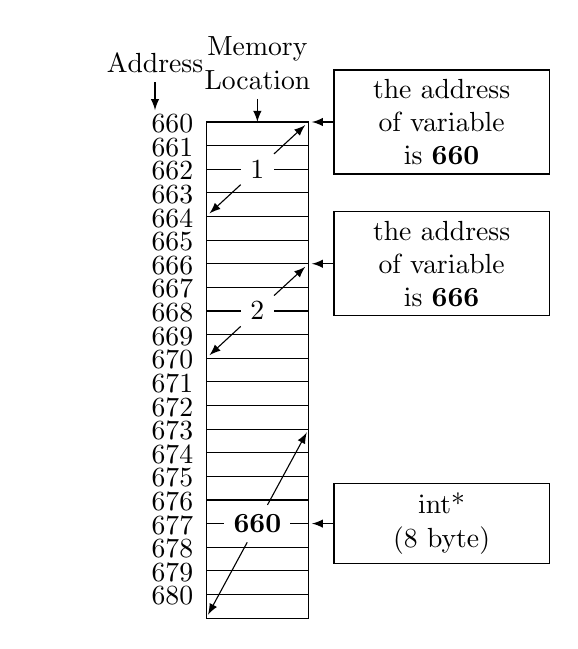
\begin{tikzpicture}[x=1.3cm,y=0.3cm]
  %% Building the boxes representing memory locations
  \foreach \x in {0,1,...,20}
  {
    \node[inner sep=1pt] (BL\x) at (0,-\x)   {};
    \node[inner sep=1pt] (UR\x) at (1,-\x+1) {};
    \node (MM\x) at ($(BL\x)!0.5!(UR\x)$) {};
    \draw (BL\x) rectangle (UR\x);
    \edef\memoryNumber{\number\numexpr660+\x\relax}
    \node[anchor=south east] at (BL\x.north west) {\memoryNumber};
  }

  %% Label columns:
  \node (MEMLOC) at ($(MM0)+(0.0,0.9cm)$) { \parbox{2cm}{\centering Memory Location} };
  \node (ADDRESS) at ($(MEMLOC)-(1.0,0)$) {\parbox{3cm}{\centering Address} };
  \draw [-latex] (MEMLOC) -- ($(MM0|-UR0)+(0.0,0)$);
  \draw [-latex] (ADDRESS) -- ($(MM0|-UR0)-(1,-0.5)$);

  %% Drawing arrows spanning memory locations
  \foreach \x/\y in {9/6}
  {
    \node[fill=white] (M\x-\y) at ($(BL\x)!0.5!(UR\y)$) {2};
    \draw[-latex]  (M\x-\y) -- (BL\x) ; 
    \draw[-latex]  (M\x-\y) -- (UR\y) ;
  }

  %% Drawing arrows spanning memory locations
  \foreach \x/\y in {3/0}
  {
    \node[fill=white] (M\x-\y) at ($(BL\x)!0.5!(UR\y)$) {1};
    \draw[-latex]  (M\x-\y) -- (BL\x) ; 
    \draw[-latex]  (M\x-\y) -- (UR\y) ;
  }

  \foreach \x/\y in {20/13}
  {
    \node [fill=white] (M\x-\y) at ($(BL\x)!0.5!(UR\y)$) {\textbf{660}};
    \draw[-latex]  (M\x-\y) -- (BL\x) ; 
    \draw[-latex]  (M\x-\y) -- (UR\y) ;
  }

  \node [draw](4byte) at ($(UR6)+(1.3,0)$) { \parbox{2.5cm}{\centering the address\\of variable\\ is \textbf{666}}};
  \path [draw,-latex] (4byte) -- (UR6);
  \node [draw](4byte) at ($(UR0)+(1.3,0)$) { \parbox{2.5cm}{\centering the address\\of variable\\ is \textbf{660}}};
  \path [draw,-latex] (4byte) -- (UR0);
  
  \node [draw](4byte) at ($(UR17)+(1.3,0)$) { \parbox{2.5cm}{\centering int* \\ (8 byte)}};
  \path [draw,-latex] (4byte) -- (UR17);

\end{tikzpicture}
    \end{column}
  \end{columns}
  
\end{frame}

\begin{frame}[fragile]
  \frametitle{Retrive the variable}
  \framesubtitle{The * operator}
  
\begin{columns}
    \begin{column}{0.55\textwidth}
    \begin{itemize}
    \item To get value, of variable, pointed by the pointer
    \item Use * operator on the pointer
    \end{itemize}
\begin{lstlisting}
int a=100;
int b=200;
int *p=&a;
printf("%d\n", *p);
\end{lstlisting}
So for \textit{int **} (pointer to pointer) the \textit{**} will give a value ...
    \end{column}
    \begin{column}{0.7\textwidth}
      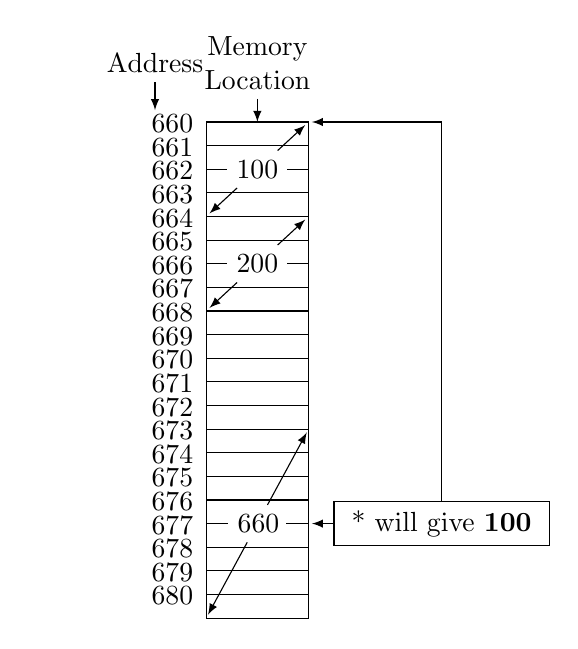
\begin{tikzpicture}[x=1.3cm,y=0.3cm]
  %% Building the boxes representing memory locations
  \foreach \x in {0,1,...,20}
  {
    \node[inner sep=1pt] (BL\x) at (0,-\x)   {};
    \node[inner sep=1pt] (UR\x) at (1,-\x+1) {};
    \node (MM\x) at ($(BL\x)!0.5!(UR\x)$) {};
    \draw (BL\x) rectangle (UR\x);
    \edef\memoryNumber{\number\numexpr660+\x\relax}
    \node[anchor=south east] at (BL\x.north west) {\memoryNumber};
  }

  %% Label columns:
  \node (MEMLOC) at ($(MM0)+(0.0,0.9cm)$) { \parbox{2cm}{\centering Memory Location} };
  \node (ADDRESS) at ($(MEMLOC)-(1.0,0)$) {\parbox{3cm}{\centering Address} };
  \draw [-latex] (MEMLOC) -- ($(MM0|-UR0)+(0.0,0)$);
  \draw [-latex] (ADDRESS) -- ($(MM0|-UR0)-(1,-0.5)$);

  %% Drawing arrows spanning memory locations
  \foreach \x/\y in {3/0}
  {
    \node[fill=white] (M\x-\y) at ($(BL\x)!0.5!(UR\y)$) {100};
    \draw[-latex]  (M\x-\y) -- (BL\x) ; 
    \draw[-latex]  (M\x-\y) -- (UR\y) ;
  }

  %% Drawing arrows spanning memory locations
  \foreach \x/\y in {7/4}
  {
    \node[fill=white] (M\x-\y) at ($(BL\x)!0.5!(UR\y)$) {200};
    \draw[-latex]  (M\x-\y) -- (BL\x) ; 
    \draw[-latex]  (M\x-\y) -- (UR\y) ;
  }

  \foreach \x/\y in {20/13}
  {
    \node [fill=white] (M\x-\y) at ($(BL\x)!0.5!(UR\y)$) {\parbox{0.5cm}{660}};
    \draw[-latex]  (M\x-\y) -- (BL\x) ; 
    \draw[-latex]  (M\x-\y) -- (UR\y) ;
  }

  \node [draw](4byte) at ($(UR17)+(1.3,0)$) { \parbox{2.5cm}{\centering * will give \textbf{100}}};
  \path [draw,-latex] (4byte) -- (UR17);
  \path [draw,-latex] (4byte) |- (UR0);
\end{tikzpicture}
    \end{column}
  \end{columns}
\end{frame}

\begin{frame}[fragile]
  \frametitle{Retrieve the variable}
  \framesubtitle{The * operator}
  
\begin{columns}
    \begin{column}{0.55\textwidth}
    \begin{itemize}
    \item To get value, of variable, pointed by the pointer
    \item Use * operator on the pointer
    \end{itemize}
\begin{lstlisting}
int a=100;
int b=200;
int *p=&a;
printf("%d\n", *p);
p=&b;
printf("%d\n", *p);
\end{lstlisting}
    \end{column}
    \begin{column}{0.7\textwidth}
      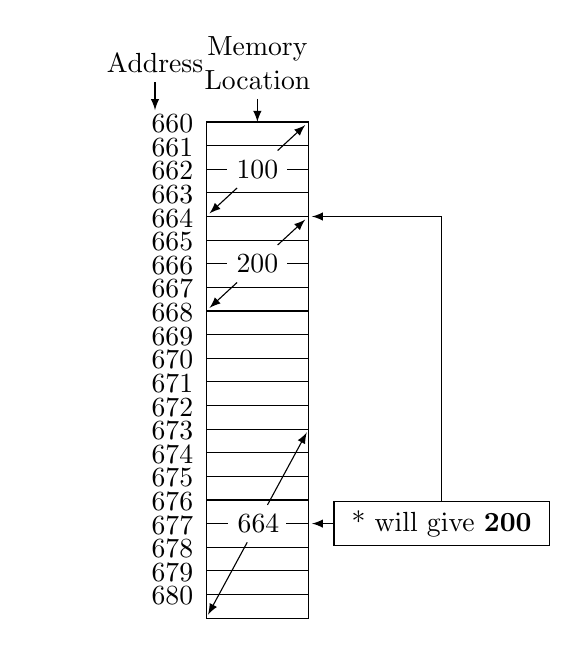
\begin{tikzpicture}[x=1.3cm,y=0.3cm]
  %% Building the boxes representing memory locations
  \foreach \x in {0,1,...,20}
  {
    \node[inner sep=1pt] (BL\x) at (0,-\x)   {};
    \node[inner sep=1pt] (UR\x) at (1,-\x+1) {};
    \node (MM\x) at ($(BL\x)!0.5!(UR\x)$) {};
    \draw (BL\x) rectangle (UR\x);
    \edef\memoryNumber{\number\numexpr660+\x\relax}
    \node[anchor=south east] at (BL\x.north west) {\memoryNumber};
  }

  %% Label columns:
  \node (MEMLOC) at ($(MM0)+(0.0,0.9cm)$) { \parbox{2cm}{\centering Memory Location} };
  \node (ADDRESS) at ($(MEMLOC)-(1.0,0)$) {\parbox{3cm}{\centering Address} };
  \draw [-latex] (MEMLOC) -- ($(MM0|-UR0)+(0.0,0)$);
  \draw [-latex] (ADDRESS) -- ($(MM0|-UR0)-(1,-0.5)$);

  %% Drawing arrows spanning memory locations
  \foreach \x/\y in {3/0}
  {
    \node[fill=white] (M\x-\y) at ($(BL\x)!0.5!(UR\y)$) {100};
    \draw[-latex]  (M\x-\y) -- (BL\x) ; 
    \draw[-latex]  (M\x-\y) -- (UR\y) ;
  }

  %% Drawing arrows spanning memory locations
  \foreach \x/\y in {7/4}
  {
    \node[fill=white] (M\x-\y) at ($(BL\x)!0.5!(UR\y)$) {200};
    \draw[-latex]  (M\x-\y) -- (BL\x) ; 
    \draw[-latex]  (M\x-\y) -- (UR\y) ;
  }

  \foreach \x/\y in {20/13}
  {
    \node [fill=white] (M\x-\y) at ($(BL\x)!0.5!(UR\y)$) {\parbox{0.5cm}{664}};
    \draw[-latex]  (M\x-\y) -- (BL\x) ; 
    \draw[-latex]  (M\x-\y) -- (UR\y) ;
  }

  \node [draw](4byte) at ($(UR17)+(1.3,0)$) { \parbox{2.5cm}{\centering * will give \textbf{200}}};
  \path [draw,-latex] (4byte) -- (UR17);
  \path [draw,-latex] (4byte) |- (UR4);
\end{tikzpicture}
    \end{column}
  \end{columns}
\end{frame}

\begin{frame}[fragile]
  \frametitle{Change the variable}
  \framesubtitle{The * operator}
  
\begin{columns}
    \begin{column}{0.55\textwidth}
    \begin{itemize}
    \item * can be used to change value pointed by the pointer
    \item Use * operator on the pointer and ...
    \end{itemize}
\begin{lstlisting}
int a=100;
int b=200;
int *p=&a;
printf("%d\n", *p);
*p = 20;
printf("%d\n", *p);
\end{lstlisting}
    \end{column}
    \begin{column}{0.7\textwidth}
      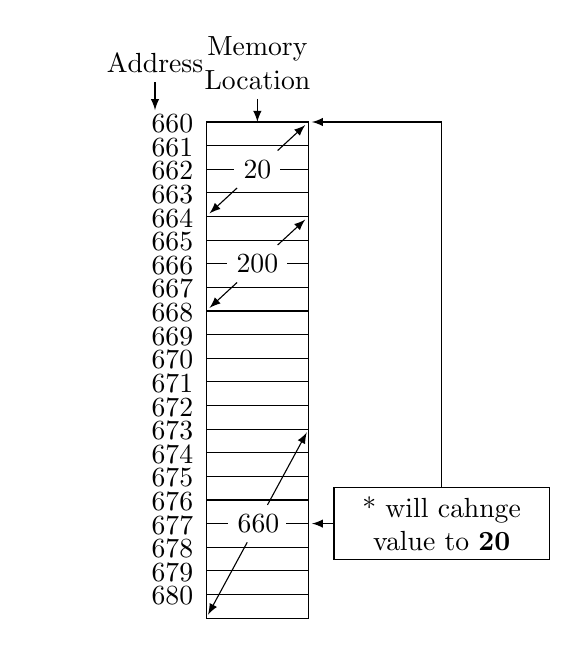
\begin{tikzpicture}[x=1.3cm,y=0.3cm]
  %% Building the boxes representing memory locations
  \foreach \x in {0,1,...,20}
  {
    \node[inner sep=1pt] (BL\x) at (0,-\x)   {};
    \node[inner sep=1pt] (UR\x) at (1,-\x+1) {};
    \node (MM\x) at ($(BL\x)!0.5!(UR\x)$) {};
    \draw (BL\x) rectangle (UR\x);
    \edef\memoryNumber{\number\numexpr660+\x\relax}
    \node[anchor=south east] at (BL\x.north west) {\memoryNumber};
  }

  %% Label columns:
  \node (MEMLOC) at ($(MM0)+(0.0,0.9cm)$) { \parbox{2cm}{\centering Memory Location} };
  \node (ADDRESS) at ($(MEMLOC)-(1.0,0)$) {\parbox{3cm}{\centering Address} };
  \draw [-latex] (MEMLOC) -- ($(MM0|-UR0)+(0.0,0)$);
  \draw [-latex] (ADDRESS) -- ($(MM0|-UR0)-(1,-0.5)$);

  %% Drawing arrows spanning memory locations
  \foreach \x/\y in {3/0}
  {
    \node[fill=white] (M\x-\y) at ($(BL\x)!0.5!(UR\y)$) {20};
    \draw[-latex]  (M\x-\y) -- (BL\x) ; 
    \draw[-latex]  (M\x-\y) -- (UR\y) ;
  }

  %% Drawing arrows spanning memory locations
  \foreach \x/\y in {7/4}
  {
    \node[fill=white] (M\x-\y) at ($(BL\x)!0.5!(UR\y)$) {200};
    \draw[-latex]  (M\x-\y) -- (BL\x) ; 
    \draw[-latex]  (M\x-\y) -- (UR\y) ;
  }

  \foreach \x/\y in {20/13}
  {
    \node [fill=white] (M\x-\y) at ($(BL\x)!0.5!(UR\y)$) {\parbox{0.5cm}{660}};
    \draw[-latex]  (M\x-\y) -- (BL\x) ; 
    \draw[-latex]  (M\x-\y) -- (UR\y) ;
  }

  \node [draw](4byte) at ($(UR17)+(1.3,0)$) { \parbox{2.5cm}{\centering * will cahnge value to \textbf{20}}};
  \path [draw,-latex] (4byte) -- (UR17);
  \path [draw,-latex] (4byte) |- (UR0);
\end{tikzpicture}
    \end{column}
  \end{columns}
\end{frame}

\begin{frame}[fragile]
  \frametitle{Change the variable}
  \framesubtitle{The * operator}
  
\begin{columns}
    \begin{column}{0.55\textwidth}
    \begin{itemize}
    \item * can be used to change value pointed by the pointer
    \item Use * operator on the pointer and ...
    \end{itemize}
\begin{lstlisting}
int a=100;
int b=200;
int *p=&a;
printf("%d\n", *p);
*p = 20;
printf("%d\n", *p);
p=&b;
*p=30;
\end{lstlisting}
    \end{column}
    \begin{column}{0.7\textwidth}
      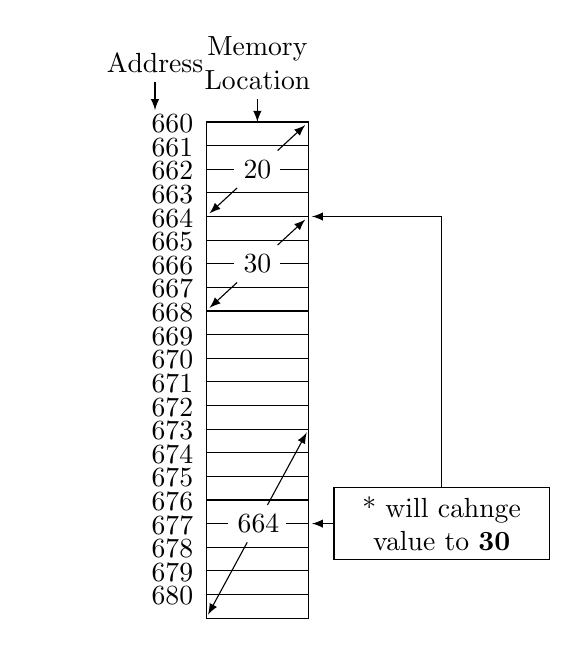
\begin{tikzpicture}[x=1.3cm,y=0.3cm]
  %% Building the boxes representing memory locations
  \foreach \x in {0,1,...,20}
  {
    \node[inner sep=1pt] (BL\x) at (0,-\x)   {};
    \node[inner sep=1pt] (UR\x) at (1,-\x+1) {};
    \node (MM\x) at ($(BL\x)!0.5!(UR\x)$) {};
    \draw (BL\x) rectangle (UR\x);
    \edef\memoryNumber{\number\numexpr660+\x\relax}
    \node[anchor=south east] at (BL\x.north west) {\memoryNumber};
  }

  %% Label columns:
  \node (MEMLOC) at ($(MM0)+(0.0,0.9cm)$) { \parbox{2cm}{\centering Memory Location} };
  \node (ADDRESS) at ($(MEMLOC)-(1.0,0)$) {\parbox{3cm}{\centering Address} };
  \draw [-latex] (MEMLOC) -- ($(MM0|-UR0)+(0.0,0)$);
  \draw [-latex] (ADDRESS) -- ($(MM0|-UR0)-(1,-0.5)$);

  %% Drawing arrows spanning memory locations
  \foreach \x/\y in {3/0}
  {
    \node[fill=white] (M\x-\y) at ($(BL\x)!0.5!(UR\y)$) {20};
    \draw[-latex]  (M\x-\y) -- (BL\x) ; 
    \draw[-latex]  (M\x-\y) -- (UR\y) ;
  }

  %% Drawing arrows spanning memory locations
  \foreach \x/\y in {7/4}
  {
    \node[fill=white] (M\x-\y) at ($(BL\x)!0.5!(UR\y)$) {30};
    \draw[-latex]  (M\x-\y) -- (BL\x) ; 
    \draw[-latex]  (M\x-\y) -- (UR\y) ;
  }

  \foreach \x/\y in {20/13}
  {
    \node [fill=white] (M\x-\y) at ($(BL\x)!0.5!(UR\y)$) {\parbox{0.5cm}{664}};
    \draw[-latex]  (M\x-\y) -- (BL\x) ; 
    \draw[-latex]  (M\x-\y) -- (UR\y) ;
  }

  \node [draw](4byte) at ($(UR17)+(1.3,0)$) { \parbox{2.5cm}{\centering * will cahnge value to \textbf{30}}};
  \path [draw,-latex] (4byte) -- (UR17);
  \path [draw,-latex] (4byte) |- (UR4);
\end{tikzpicture}
    \end{column}
  \end{columns}
\end{frame}

\begin{frame}[fragile]
  \frametitle{Printing the address stored by a pointer}
  \framesubtitle{\%p ... or \%d}
\begin{lstlisting}
int a=10;
printf("%p\n", &a);
int *p = &a;
printf("%p\n", p)

printf("%p\n", &p);??
\end{lstlisting}
\end{frame}

\begin{frame}[fragile]
  \frametitle{Pointer arithmetic}
  \framesubtitle{+ -}
\begin{lstlisting}
int a=10;
printf("%p\n", &a);
int *p = &a;
printf("%p\n", p+1)?
\end{lstlisting}

How many \textit{ints} I could hide in a single \textit{double} ...\\
I should not ...

\end{frame}

\section{Revisiting functions}

\begin{frame}[fragile]
  \frametitle{Function with arguments}
  \framesubtitle{Passed by value}
\begin{columns}
    \begin{column}{0.55\textwidth}
    \begin{itemize}
    \item Only the value is send to a function
    \end{itemize}
\begin{lstlisting}
void fun(int a){
  a = 500;
}

int main(){
  inb b=20;
  fun(b);
  //b?
}
\end{lstlisting}
    \end{column}
    \begin{column}{0.7\textwidth}
      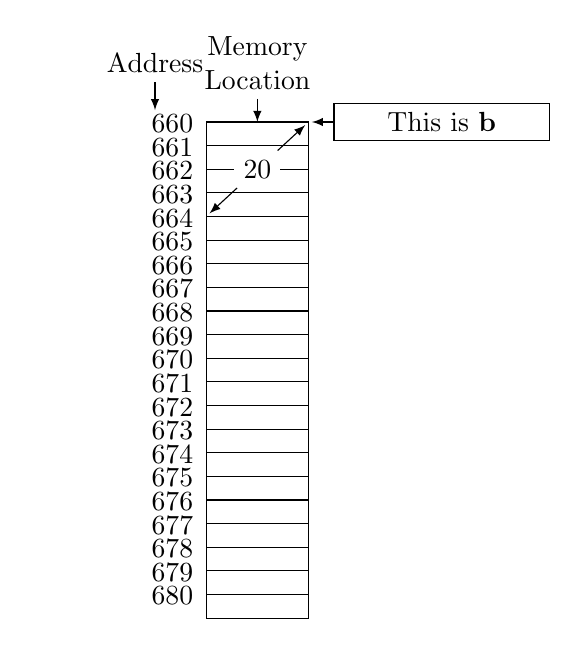
\begin{tikzpicture}[x=1.3cm,y=0.3cm]
  %% Building the boxes representing memory locations
  \foreach \x in {0,1,...,20}
  {
    \node[inner sep=1pt] (BL\x) at (0,-\x)   {};
    \node[inner sep=1pt] (UR\x) at (1,-\x+1) {};
    \node (MM\x) at ($(BL\x)!0.5!(UR\x)$) {};
    \draw (BL\x) rectangle (UR\x);
    \edef\memoryNumber{\number\numexpr660+\x\relax}
    \node[anchor=south east] at (BL\x.north west) {\memoryNumber};
  }

  %% Label columns:
  \node (MEMLOC) at ($(MM0)+(0.0,0.9cm)$) { \parbox{2cm}{\centering Memory Location} };
  \node (ADDRESS) at ($(MEMLOC)-(1.0,0)$) {\parbox{3cm}{\centering Address} };
  \draw [-latex] (MEMLOC) -- ($(MM0|-UR0)+(0.0,0)$);
  \draw [-latex] (ADDRESS) -- ($(MM0|-UR0)-(1,-0.5)$);

  %% Drawing arrows spanning memory locations
  \foreach \x/\y in {3/0}
  {
    \node[fill=white] (M\x-\y) at ($(BL\x)!0.5!(UR\y)$) {20};
    \draw[-latex]  (M\x-\y) -- (BL\x) ; 
    \draw[-latex]  (M\x-\y) -- (UR\y) ;
  }

  \node [draw](4byte) at ($(UR0)+(1.3,0)$) { \parbox{2.5cm}{\centering This is \textbf{b}}};
  \path [draw,-latex] (4byte) -- (UR0);
\end{tikzpicture}
\end{column}
\end{columns}
\end{frame}

\begin{frame}[fragile]
  \frametitle{Function with arguments}
  \framesubtitle{Passed by value}
\begin{columns}
    \begin{column}{0.55\textwidth}
    \begin{itemize}
    \item Only the value is send to a function
    \end{itemize}
\begin{lstlisting}
void fun(int a){
  a = 500;
}

int main(){
  inb b=20;
  fun(b);
  //b?
}
\end{lstlisting}
    \end{column}
    \begin{column}{0.7\textwidth}
      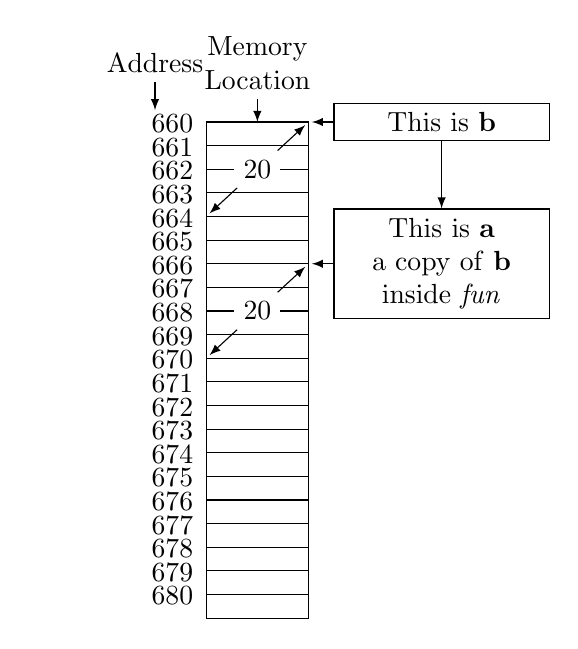
\begin{tikzpicture}[x=1.3cm,y=0.3cm]
  %% Building the boxes representing memory locations
  \foreach \x in {0,1,...,20}
  {
    \node[inner sep=1pt] (BL\x) at (0,-\x)   {};
    \node[inner sep=1pt] (UR\x) at (1,-\x+1) {};
    \node (MM\x) at ($(BL\x)!0.5!(UR\x)$) {};
    \draw (BL\x) rectangle (UR\x);
    \edef\memoryNumber{\number\numexpr660+\x\relax}
    \node[anchor=south east] at (BL\x.north west) {\memoryNumber};
  }

  %% Label columns:
  \node (MEMLOC) at ($(MM0)+(0.0,0.9cm)$) { \parbox{2cm}{\centering Memory Location} };
  \node (ADDRESS) at ($(MEMLOC)-(1.0,0)$) {\parbox{3cm}{\centering Address} };
  \draw [-latex] (MEMLOC) -- ($(MM0|-UR0)+(0.0,0)$);
  \draw [-latex] (ADDRESS) -- ($(MM0|-UR0)-(1,-0.5)$);

  %% Drawing arrows spanning memory locations
  \foreach \x/\y in {3/0}
  {
    \node[fill=white] (M\x-\y) at ($(BL\x)!0.5!(UR\y)$) {20};
    \draw[-latex]  (M\x-\y) -- (BL\x) ; 
    \draw[-latex]  (M\x-\y) -- (UR\y) ;
  }
  
  %% Drawing arrows spanning memory locations
  \foreach \x/\y in {9/6}
  {
    \node[fill=white] (M\x-\y) at ($(BL\x)!0.5!(UR\y)$) {20};
    \draw[-latex]  (M\x-\y) -- (BL\x) ; 
    \draw[-latex]  (M\x-\y) -- (UR\y) ;
  }

  \node [draw](b) at ($(UR0)+(1.3,0)$) { \parbox{2.5cm}{\centering This is \textbf{b}}};
  \path [draw,-latex] (b) -- (UR0);
  \node [draw](a) at ($(UR6)+(1.3,0)$) { \parbox{2.5cm}{\centering This is \textbf{a}\\a copy of \textbf{b}\\inside \textit{fun}}};
  \path [draw,-latex] (a) -- (UR6);
  \path [draw,-latex] (b) -- (a);
\end{tikzpicture}
\end{column}
\end{columns}
\end{frame}

\begin{frame}[fragile]
  \frametitle{Function with arguments}
  \framesubtitle{Passed by value}
\begin{columns}
    \begin{column}{0.55\textwidth}
    \begin{itemize}
    \item Only the value is send to a function
    \end{itemize}
\begin{lstlisting}
void fun(int a){
  a = 500;
}

int main(){
  inb b=20;
  fun(b);
  //b?
}
\end{lstlisting}
    \end{column}
    \begin{column}{0.7\textwidth}
      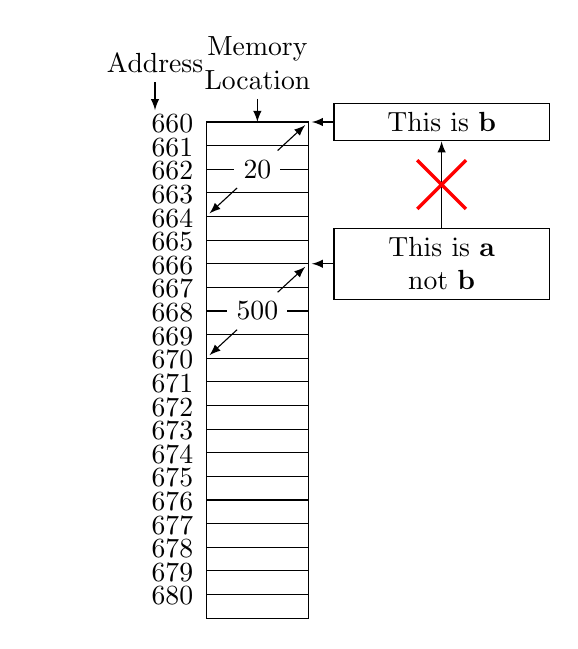
\begin{tikzpicture}[x=1.3cm,y=0.3cm]
  %% Building the boxes representing memory locations
  \foreach \x in {0,1,...,20}
  {
    \node[inner sep=1pt] (BL\x) at (0,-\x)   {};
    \node[inner sep=1pt] (UR\x) at (1,-\x+1) {};
    \node (MM\x) at ($(BL\x)!0.5!(UR\x)$) {};
    \draw (BL\x) rectangle (UR\x);
    \edef\memoryNumber{\number\numexpr660+\x\relax}
    \node[anchor=south east] at (BL\x.north west) {\memoryNumber};
  }

  %% Label columns:
  \node (MEMLOC) at ($(MM0)+(0.0,0.9cm)$) { \parbox{2cm}{\centering Memory Location} };
  \node (ADDRESS) at ($(MEMLOC)-(1.0,0)$) {\parbox{3cm}{\centering Address} };
  \draw [-latex] (MEMLOC) -- ($(MM0|-UR0)+(0.0,0)$);
  \draw [-latex] (ADDRESS) -- ($(MM0|-UR0)-(1,-0.5)$);

  %% Drawing arrows spanning memory locations
  \foreach \x/\y in {3/0}
  {
    \node[fill=white] (M\x-\y) at ($(BL\x)!0.5!(UR\y)$) {20};
    \draw[-latex]  (M\x-\y) -- (BL\x) ; 
    \draw[-latex]  (M\x-\y) -- (UR\y) ;
  }
  
  %% Drawing arrows spanning memory locations
  \foreach \x/\y in {9/6}
  {
    \node[fill=white] (M\x-\y) at ($(BL\x)!0.5!(UR\y)$) {500};
    \draw[-latex]  (M\x-\y) -- (BL\x) ; 
    \draw[-latex]  (M\x-\y) -- (UR\y) ;
  }

  \node [draw](b) at ($(UR0)+(1.3,0)$) { \parbox{2.5cm}{\centering This is \textbf{b}}};
  \path [draw,-latex] (b) -- (UR0);
  \node [draw](a) at ($(UR6)+(1.3,0)$) { \parbox{2.5cm}{\centering This is \textbf{a}\\not \textbf{b}}};
  \path [draw,-latex] (a) -- (UR6);
  \tikzset{cross/.style={cross out, draw=black, minimum size=2*(#1-\pgflinewidth),
  inner sep=0pt, outer sep=0pt, very thick}, cross/.default={10pt}}
  \path [draw,-latex] (a) -- node[cross, red] (c) {} (b);
\end{tikzpicture}
\end{column}
\end{columns}
\end{frame}

\begin{frame}[fragile]
  \frametitle{Function with arguments}
  \framesubtitle{Pass an address?}
\begin{columns}
    \begin{column}{0.55\textwidth}
    \begin{itemize}
    \item What if we pass an address to a variable
    \item Than the function "knows" where the variable is stored
    \item The function works on tha variable
    \item ... not a copy
    \end{itemize}
\begin{lstlisting}
void fun(int* a){
  *a = 500;
}

int main(){
  inb b=20;
  fun(&b);//like scanf
  //b?
}
\end{lstlisting}
    \end{column}
    \begin{column}{0.7\textwidth}
      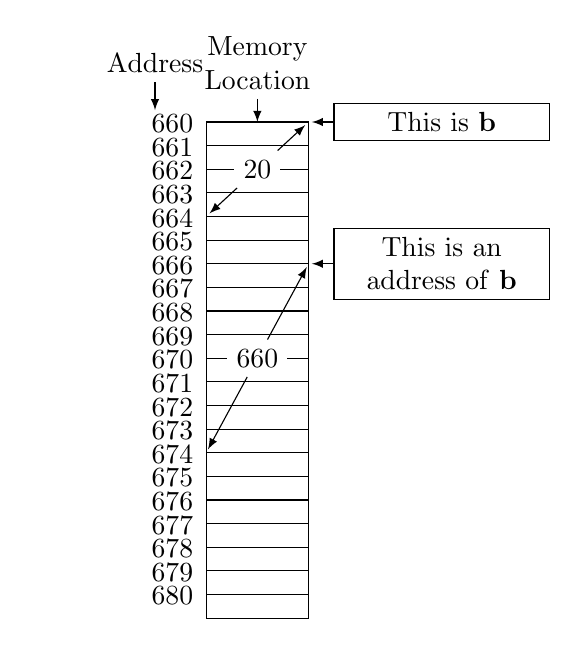
\begin{tikzpicture}[x=1.3cm,y=0.3cm]
  %% Building the boxes representing memory locations
  \foreach \x in {0,1,...,20}
  {
    \node[inner sep=1pt] (BL\x) at (0,-\x)   {};
    \node[inner sep=1pt] (UR\x) at (1,-\x+1) {};
    \node (MM\x) at ($(BL\x)!0.5!(UR\x)$) {};
    \draw (BL\x) rectangle (UR\x);
    \edef\memoryNumber{\number\numexpr660+\x\relax}
    \node[anchor=south east] at (BL\x.north west) {\memoryNumber};
  }

  %% Label columns:
  \node (MEMLOC) at ($(MM0)+(0.0,0.9cm)$) { \parbox{2cm}{\centering Memory Location} };
  \node (ADDRESS) at ($(MEMLOC)-(1.0,0)$) {\parbox{3cm}{\centering Address} };
  \draw [-latex] (MEMLOC) -- ($(MM0|-UR0)+(0.0,0)$);
  \draw [-latex] (ADDRESS) -- ($(MM0|-UR0)-(1,-0.5)$);

  %% Drawing arrows spanning memory locations
  \foreach \x/\y in {3/0}
  {
    \node[fill=white] (M\x-\y) at ($(BL\x)!0.5!(UR\y)$) {20};
    \draw[-latex]  (M\x-\y) -- (BL\x) ; 
    \draw[-latex]  (M\x-\y) -- (UR\y) ;
  }
  
  %% Drawing arrows spanning memory locations
  \foreach \x/\y in {13/6}
  {
    \node[fill=white] (M\x-\y) at ($(BL\x)!0.5!(UR\y)$) {660};
    \draw[-latex]  (M\x-\y) -- (BL\x) ; 
    \draw[-latex]  (M\x-\y) -- (UR\y) ;
  }

  \node [draw](b) at ($(UR0)+(1.3,0)$) { \parbox{2.5cm}{\centering This is \textbf{b}}};
  \path [draw,-latex] (b) -- (UR0);
  \node [draw](a) at ($(UR6)+(1.3,0)$) { \parbox{2.5cm}{\centering This is an address of \textbf{b}}};
  \path [draw,-latex] (a) -- (UR6);
\end{tikzpicture}
\end{column}
\end{columns}
\end{frame}

\begin{frame}[fragile]
  \frametitle{Function with arguments}
  \framesubtitle{Pass an address?}
\begin{columns}
    \begin{column}{0.55\textwidth}
    \begin{itemize}
    \item What if we pass an address to a variable
    \item Than the function "knows" where the variable is stored
    \item The function works on tha variable
    \item ... not a copy
    \end{itemize}
\begin{lstlisting}
void fun(int* a){
  *a = 500;
}

int main(){
  inb b=20;
  fun(&b);//like scanf
  //b?
}
\end{lstlisting}
    \end{column}
    \begin{column}{0.7\textwidth}
      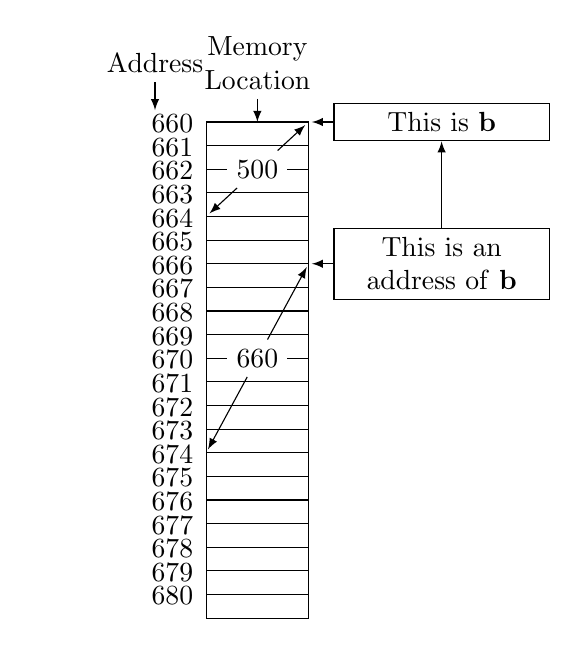
\begin{tikzpicture}[x=1.3cm,y=0.3cm]
  %% Building the boxes representing memory locations
  \foreach \x in {0,1,...,20}
  {
    \node[inner sep=1pt] (BL\x) at (0,-\x)   {};
    \node[inner sep=1pt] (UR\x) at (1,-\x+1) {};
    \node (MM\x) at ($(BL\x)!0.5!(UR\x)$) {};
    \draw (BL\x) rectangle (UR\x);
    \edef\memoryNumber{\number\numexpr660+\x\relax}
    \node[anchor=south east] at (BL\x.north west) {\memoryNumber};
  }

  %% Label columns:
  \node (MEMLOC) at ($(MM0)+(0.0,0.9cm)$) { \parbox{2cm}{\centering Memory Location} };
  \node (ADDRESS) at ($(MEMLOC)-(1.0,0)$) {\parbox{3cm}{\centering Address} };
  \draw [-latex] (MEMLOC) -- ($(MM0|-UR0)+(0.0,0)$);
  \draw [-latex] (ADDRESS) -- ($(MM0|-UR0)-(1,-0.5)$);

  %% Drawing arrows spanning memory locations
  \foreach \x/\y in {3/0}
  {
    \node[fill=white] (M\x-\y) at ($(BL\x)!0.5!(UR\y)$) {500};
    \draw[-latex]  (M\x-\y) -- (BL\x) ; 
    \draw[-latex]  (M\x-\y) -- (UR\y) ;
  }
  
  %% Drawing arrows spanning memory locations
  \foreach \x/\y in {13/6}
  {
    \node[fill=white] (M\x-\y) at ($(BL\x)!0.5!(UR\y)$) {660};
    \draw[-latex]  (M\x-\y) -- (BL\x) ; 
    \draw[-latex]  (M\x-\y) -- (UR\y) ;
  }

  \node [draw](b) at ($(UR0)+(1.3,0)$) { \parbox{2.5cm}{\centering This is \textbf{b}}};
  \path [draw,-latex] (b) -- (UR0);
  \node [draw](a) at ($(UR6)+(1.3,0)$) { \parbox{2.5cm}{\centering This is an address of \textbf{b}}};
  \path [draw,-latex] (a) -- (UR6);
  \path [draw,-latex] (a) -- (b);
  
\end{tikzpicture}
\end{column}
\end{columns}
\end{frame}

\end{document}
